\documentclass[heading.tex]{subfiles} 
\begin{document}

% \tableofcontents

\section{Introduction and Motivation}
Historically, there have been completely separate code-bases for design space exploration and
transient engine analysis. The capability to create flexible ``low fidelity'' models is ideal in
the earliest  conceptual design stages, where large design spaces can be explored relatively
quickly. As the engine design starts to become more concrete, higher fidelity models are
developed. These higher detail models are intrinsically more sensitive to design tweaks, and in
general take longer to setup. They inherently require more stringently defined configurations
and boundary conditions. A large variation in the baseline design could
potentially render entire higher fidelity analyses obsolete. Due to this weakness in adaptability,
higher fidelity models are generally not created until the low-fidelity design has fully matured.
This friction can partly be attributed to the differences in toolstes when transitioning to higher
fidelity models. 

\subsection{Design Cycle Overview}

	From a life-cycle perspective, there comes a point when the prospect of re-design becomes
prohibitively expensive and initial design decisions become cemented into the design. Any insights
gained from more detailed analyses are constrained to these initial design choices. Naturally, a
tradeoff exists on the amount of time spent in each analysis phase. Spending more time in the low
fidelity phase could have large payoffs in the long run; however, without higher fidelity models
it is hard to identify possible shortcomings such as those arising from operability and control
issues.

\begin{figure}[H]
\centering
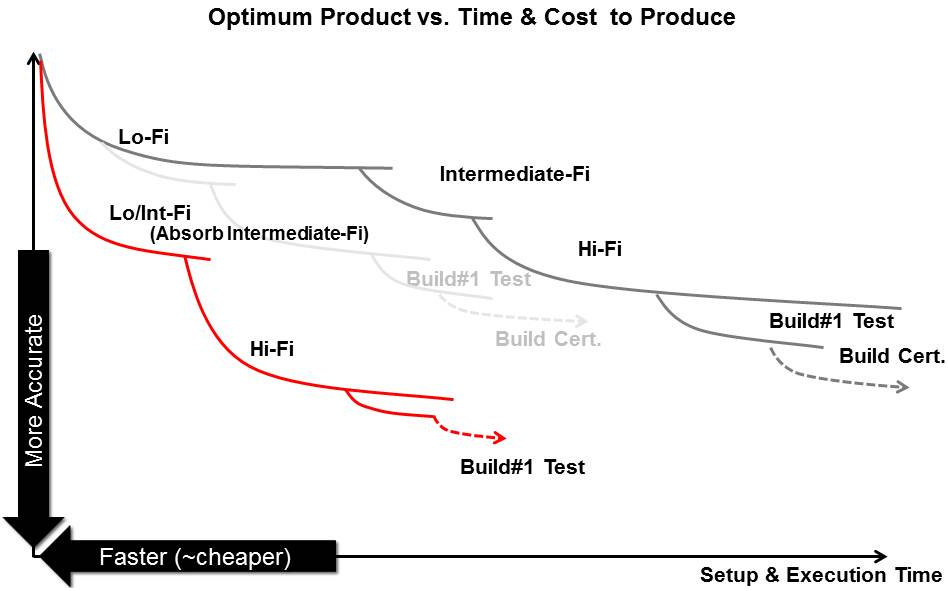
\includegraphics[width=1.0\textwidth]{images/optimum_product_vs_time}
\caption{Overarching Applied Research Challenge: Uncertainty in Optimum Product vs. Time \& Cost to Produce}
\label{f:product_vs_time}
\end{figure}

Figure \ref{f:product_vs_time} shows a pedagogical representation of the general relation between
accuracy and analysis set-up time, with the origin representing the perfect analysis capability.
Lower fidelity (Lo-Fi) models are less accurate, but can be set
up and modified relatively quickly. The darker gray path characterizes the tradtional design
trend. Higher fidelity (Hi-Fi) models take longer to build, and therefore, aren't started until
the low fidelity design reaches quiescence. If designers attempt to introduce Hi-Fi models earlier in
the design, as shown by the light gray line shifted to the left, they quickly become outdated as
the baseline model continues to undergo changes. Inevitably the models must be re-written to match
the new Lo-Fi design and the path reverts to the dark gray route. The only way to incorporate the
intermediate fidelity model earlier into the design process, is by absorbing the Int-Fi codes into
the low fidelity codes as portrayed by the red line. Combining both disciplines into a unified code
would accomplish this, but each toolset can remain distinct as long as the Int-Fi model is
adaptable enough to keep up with the rapid changes of the Low-Fi code.
Creating a single unified program to satisfy every design need runs an equally high risk
of becoming overly complex or cumbersome. 
A natural reaction is for various
disciplines to diverge and create unique tools satisfying their particular needs using frameworks
and programming languages that are already of familiarity. As mentioned earlier, this is
acceptable as long as the codes preserve flexibility and rapid adaptability. An intermediate
fidelity code can only be introduced earlier into the low fidelity analysis phase if it can keep
pace with the rapid redesigns.

The subsequent sections explore various design patterns to rapidly develop transient models. Each
approach starts with a base model built with NPSS, and assumes the reader already has a basic
understanding of how to construct a steady-state model. This paper focuses on further enhancements
required to interface NPSS with Matlab codes. The first method being the simplest and most
straightforward but performance constrained. The last being the most abstract. These methods
aren't mutually exclusive and the specific implementation details could vary greatly based on the
designer's discretion. 


\section{Running NPSS Transiently}

This paper assumes a basic understanding of the concepts required for steady-state engine modeling within NPSS.
Foundational concepts are best introduced in the NPSS user's guide \cite{NPSS} and other introductory resources.
\cite{JonesIntro} 
Transient simulations represent the time-varying behavior of a system by finding a series of
solutions at discrete time steps over a desired time interval. NPSS solves these systems of
equations largely in the same way it handles steady-state solutions. However for transient
systems, some of the equations require engine state integration rather than simply driving imbalances to zero.


\subsection{Solver and Integration Methods}
NPSS supports multiple integration types that are outlined in the NPSS users guide.
\cite[chap.~7.1]{NPSS} Table \ref{tab:Integration} summarizes the available methods, with a 
first-order differential equation for spool speed used as an example: 

\begin{minipage}{\linewidth}
\centering
\bigskip
\captionof{table}{NPSS Integration Methods} \label{tab:Integration}
\begin{tabular}{|c|c|c|}
\hline 
Method & Type & Solving for  $N_{t2}$, given  $N_{t2}- N_{t1}= \int_{t1}^{t2} \! \dfrac{T_{net}}{I} \, \mathrm{d}t $\\ 
\hline 
Euler & Explicit & $ \left.N_{t2}= N_{t1} + \dfrac{T_{net}}{I} \right|_{t1}^{}(t2-t1)$ \\ 
\hline 
Trapezoidal & Implicit & $ \left.N_{t2}= N_{t1} + \dfrac{1}{2}\middle(\dfrac{T_{net}}{I} \middle|_{t1}^{}+\dfrac{T_{net}}{I} \middle|_{t2}^{}\right)(t2-t1)$ \\ 
\hline 
$1^{st}$ Order Gear & Implicit & $ \left.N_{t2}= N_{t1} + \dfrac{ \mathrm{d}N }{ \mathrm{d}t } \right|_{t2}^{}(t2-t1)$ \\ 
\hline 
$2^{nd}$ Order Gear & Implicit & $ \left.N_{t2}= N_{t1} + \middle(\dfrac{1}{3}\dfrac{ \mathrm{d}N }{ \mathrm{d}t }\middle|_{t1}^{}+\dfrac{2}{3}\dfrac{ \mathrm{d}N }{ \mathrm{d}t }\middle|_{t2}^{}\right)(t2-t1)$ \\ 
\hline 
\end{tabular} 
\end{minipage}

Steady-state iteration may be required for any of these methods, and the choice between explicit
and implicit types comes down to accuracy vs time. Explicit methods assume the integrand is
constant over the specified time interval, therefore integration is only performed once per time
step. Implicit methods perform a sub-iteration (independent from time) until the predicted state
value agrees with the corrected value within a specified tolerance. NPSS also allows the user to
define custom integration methods using the \texttt{Integrator} class. \cite[chap.~15.2]{NPSS}  

\begin{adjustwidth}{-0.5cm}{-0.5cm}
 \begin{minted}{c++}
 setOption( "solutionMode", "TRANSIENT" );
 Transient.integrationType = "TRAPEZOIDAL"; //Default Gear 1st order
 transient.setup(); //run if changing to (or from) Euler method
 initializeHistory(); //run if initial conditions 
 	//differ from most recent transient run
 \end{minted}
 \end{adjustwidth} 
       

The top level transient solver is of type \texttt{TransientExecutive}, and is named
\texttt{transient} by default. This variable is analogous to the top-level steady-state 
``\texttt{solver}" object. The \texttt{transient} object is responsible for setting integration
solver properties including the simulation start, step and stop parameters. \cite[chap.~7.5]{NPSS}
\cite[chap.~15.1.8]{NPSS}  All attributes have a default value except \texttt{transient.stopTime},
which must be supplied by the user. Over the course of a run, the \texttt{TransientExecutive} may
update these attributes or even overwrite values set by the user. The user can also preemptively
stop a simulation using the  \texttt{quiescence()} and  \texttt{terminateCondition()} functions
available in the \texttt{TransientExecutive}.

\begin{adjustwidth}{0cm}{0cm}
 \begin{minted}{c++}
transient { //set as a group
	timeStepMethod = "ADAPTIVE";
	baseTimeStep= 0.10;
	dxTransLimit = 0.05;
	maxTimeStep = 0.20;
	minTimeStep = 0.01;
	stopTime= 3.60;
} //or set individually: transient.stopTime = 3.6;
 \end{minted}
 \end{adjustwidth} 

Before running transiently, the user must first ensure that each engine component with transient
specific attributes is properly initialized. Common components with special transient properties
include, shafts, springs, control volumes, heat exchangers, walls and thermal masses.
The following code snippet shows how the special \texttt{inertia} property may be initialized
for a shaft component:

 \begin{adjustwidth}{-1cm}{-1cm}
 \inputminted[]{c++}{code/shaft.mdl}
 \end{adjustwidth} 

In steady-state mode, the solver will vary the shaft's mechanical speed to
balance the input turbine torques with the output compressor port torques.
In transient mode, the shaft speed is varied until the speed
controlled by the solver is equal to the speed calculated by integrating
the acceleration derived from the net engine torque.

\subsection{Transient Dependents and Constraints}

Time-varying inputs, dependents, and constraints must be defined and evaluated at every time step during a simulation, and therefore cannot simply be
assigned to a constant value before executing the \texttt{run()} command. Time dependent variables can be calculated explicitly with
piecewise functions for every time step or scheduled using built-in table and interpolation routines.
The code snippets below show both of these methods respectively, for defining fuel flow as shown in figure \ref{f:ramp}.

\begin{figure}[H]
\centering
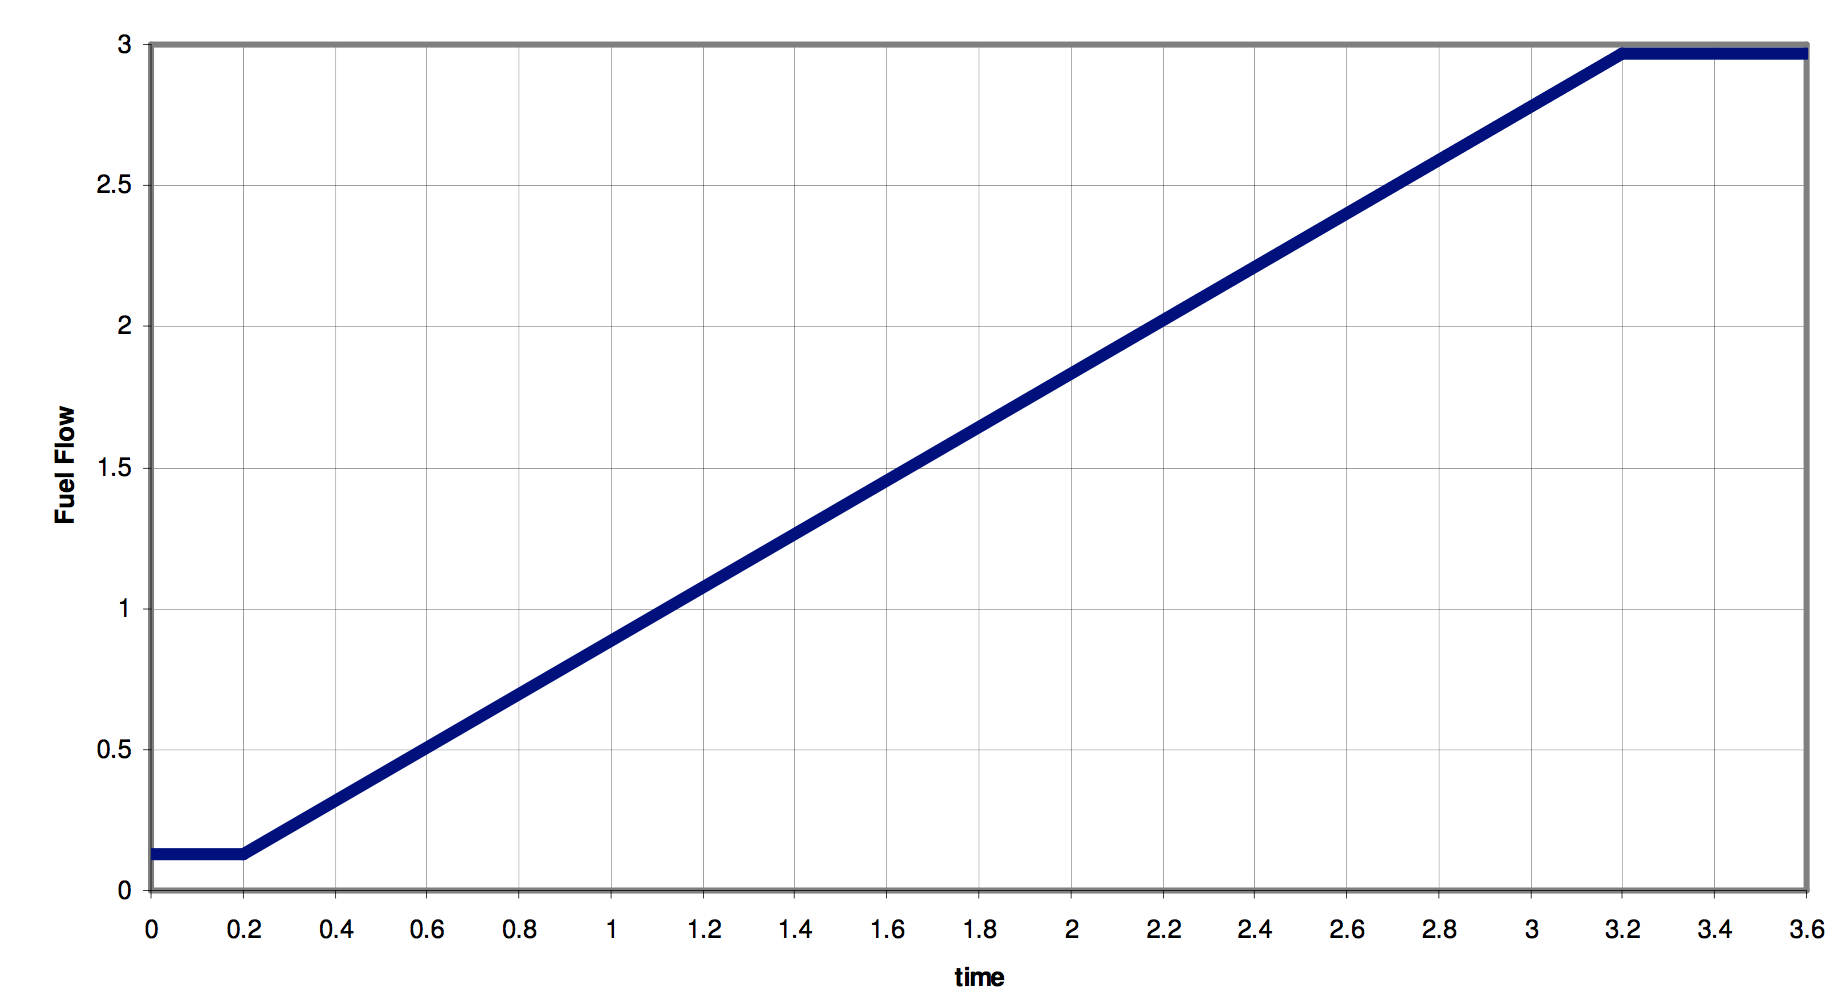
\includegraphics[width=1.0\textwidth]{images/fuelRamp}
\caption{Example fuel ramp used to drive a transient run}
\label{f:ramp}
\end{figure}

\begin{adjustwidth}{-1cm}{-1cm}
 \inputminted[]{c++}{code/rampFn}
 \end{adjustwidth} 
 
Or the same function could be built using a table. 
 
 \begin{adjustwidth}{-1cm}{-1cm}
 \inputminted[]{c++}{code/rampTb}
 \end{adjustwidth} 

The last line of each of these example functions tells NPSS how to evaluate the calculated fuel flow input.
These dynamic variables can evaluated by creating a set of independent/dependent equations as show below.
The transient variable function is set as the right hand side (\texttt{rhs}) of a dependent equation,
with the left hand side (\texttt{lhs}) set to fuel flow. 
A second variable must be defined as the independent variable and is varied by the solver until the dependent
equation is satisfied.
The independent variable and \texttt{eq\_lhs} dependent variable don't necessarily have to be the same
as shown in this example. However, the independent variable must be able to indirectly influence the
value of the dependent \texttt{eq\_lhs}.

 \begin{adjustwidth}{1cm}{-1cm}
 \inputminted[]{c++}{code/solverSetup}
 \end{adjustwidth} 


Multiple dependent equations can be paired with a single independent variable in the form of constraints.
This method is appropriate when the user intends to drive an output variable transiently,
such as thrust, while ensuring no engine constraints are violated.
This behavior can be beneficial for simulating engine limiters in a controller, and managing 
competing constraints on several variables.
 
 \begin{adjustwidth}{1cm}{-1cm}
 \inputminted[]{c++}{code/constraintSetup}
 \end{adjustwidth} 
 
Although the constraint is defined identically to a dependent variable, it is applied to a pre-existing independent variable.
The example shown above varies fuel flow to reach a specified thrust target, but only as long as a temperature constraint isn't violated.
As long as this constraint is activated, fuel flow will follow the temperature limit and ignore the thrust target.
Since numerous constraints can be applied to a dependent variable,
optional arguments can be supplied to specify if a variable is a minimum or maximum limit.
The optional third argument of the \texttt{addConstraint} method, labeled as `priority' in the code snippet above,
determines which limit to ignore if competing min and max limits are violated.
In rare cases, the change in error is negatively correlated to changes in the independent variable,
leading to the solver to get locked into alternating limits. One such case would be varying fuel flow to reach a target thrust,
with an additional constraint on minimum and maximum low pressure compressor Rlines.
Flipping the `MIN' or `MAX' and the sign of the `slope' arguments can be used to resolve this numerical instability.

A further abstracted method of setting user defined variables can be implemented using the NPSS supplied 
\texttt{solversequence()} method.
This allows users to simply append a function to the beginning or end of every time-step calculation loop
and evaluate any variable to a specified value. 
 
 \begin{adjustwidth}{-1cm}{-1cm}
 \inputminted[]{c++}{code/solverSequence}
 \end{adjustwidth} 
 
This code block performs a functionally equivalent operation to the first example snippet of this section.
Although the computational differences are minor, this provides the user with another option for organizing logic.
From an organizational standpoint,
it may be desirable to fully separate concerns by keeping certain logic separate from the model itself.
Example code demonstrating all of these methods can be found in \cref{app:transient}.

\subsection{Transient Output}

In order to capture the engine state after convergence of every time step, standard viewers or custom functions can be
invoked for transient cases using the \texttt{solver} \texttt{.postExecutionSequence} method. This method takes an array of strings that
correspond to viewer objects or function names. If a PageViewer or DataViewer is called, it will automatically invoke the
\texttt{display()} method of these objects, if a CaseViewer is called, only the \texttt{update()} method will be invoked.
If an implicit integration method is used, the viewer will only update after each sub-iteration is fully converged.

 \begin{adjustwidth}{-1cm}{-1cm}
 \inputminted[]{c++}{code/transient1}
 \end{adjustwidth} 

Additional viewer reference material can be found in \cite[chap.~7.2.2, ~12, ~15.3.1]{NPSS}

\subsection{Transient Run Files}

In summary, a transient model generally requires the minimum following steps:

\begin{enumerate}
\item Defining transient engine components and initial conditions for transient-specific properties
\item Defining time-varying input/output variables using functions or interpolation tables,
which are are subsequently connected to the solver via independents, dependents, and constraints
\item Configuring transient solver parameters: solutionMode, time boundary, time step, tolerances, termination criteria
\item Configuring output viewers
\end{enumerate}

It's generally recommended to organize each of these steps in separate files or folders to better manage complexity.
Each aspect is then generally orchestrated in a run file containing numerous simulations chained together. 
After steady-state engine sizing occurs, engine state boundaries can be established by running multiple
off-design power settings until key engine constraints become active. Generating large tables of equilibrated or `trimmed' engine points
throughout the flight envelopes ensures that transients can be run from any starting condition without
starting imbalances.
In the following example, a steady-state case is first run to initialize the state of the engine and
to determine fuel flow bounds on a transient input driver based on user-provided thrust targets.
A transient case is then run from t=0 to t=0.6, paused, then resumed to t=3.6.
Finally, a new transient run clears the previously integrated engine states and runs a fresh case from t=0 to t=2.4.

 \begin{adjustwidth}{1cm}{-1cm}
 \inputminted[]{c++}{code/transientRun}
 \end{adjustwidth} 

\subsection{Advanced Dynamics Modeling}

Users can find additional transient solver options in the NPSS user's guide \cite[chap.~18]{NPSS} for simulating
more advanced engine dynamics such as custom first order-lags, adaptive time-stepping, custom integrators or
predictor calculations.

While possible to implement in NPSS, many advanced modeling processes are can benefit
from specialized toolsets in other development environments such as Matlab/Simulink.
The following sections outline strategies for interfacing NPSS with Matlab to take advantage of Matlab's large
ecosystem of tools.

\section{Passing Data Between NPSS and Matlab}
\subsection{Raw File I/O}

The most simplistic and straightforward method for passing information is automated
file passing and batched system calls.

File I/O is undesirable from a performance aspect, but can be acceptable if the total number of round-trips between
NPSS and Matlab are minimized. This method is suitable for upfront engine initialization calculations, 
and functions where programming simplicity is more important than computational efficiency.

A single round-trip generally involves the following steps:

\begin{figure}[H]
\centering
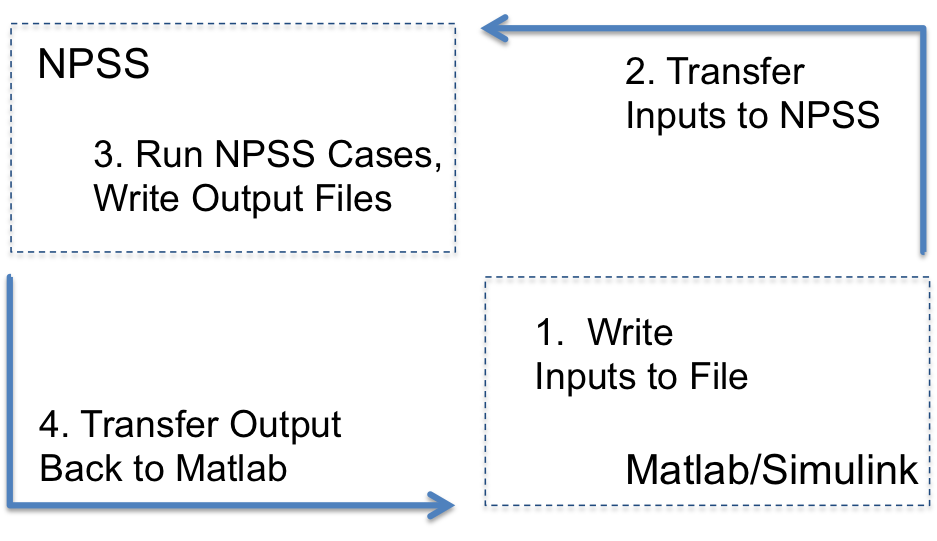
\includegraphics[width=0.5\textwidth]{images/roundTrip}
\caption{Example DataFlow for File I/O}
\label{f:DialogBox}
\end{figure}

\begin{enumerate}
  \item Specify run cases, programatically writing the necessary batch and input files $[Matlab]$
  \item Transfer cases to the NPSS model directory $[Matlab \rightarrow NPSS]$
  \item Execute NPSS Run Cases, saving output variables of interest in a matlab readable syntax $[NPSS]$
  \item Transfer output files back to Matlab where they can be loaded into the working directory $[NPSS \rightarrow Matlab]$
\end{enumerate}


Matlab can dynamically write input/run scripts, which are subsequently
copied to the NPSS directory and executed from a system call.
The following template generates an input file

 \begin{adjustwidth}{-1cm}{-1cm}
 \inputminted[]{matlab}{code/dlmwrite.m}
 \end{adjustwidth} 

which will create the following file, called \texttt{NPSS\_setpoint.input}

 \begin{adjustwidth}{-1cm}{-1cm}
 \inputminted[]{matlab}{code/dlmOutput.m}
 \end{adjustwidth} 


This method works best when adhering to a few hueristics. Firstly, organize an engine repository
into subfolders. Although it's possible to contain everything within a single file, separating code
improves readability and simplifies automated file operations when they can be limited to a smaller subset of files.
Table \ref{tab:Scaffolding} shows one such way to organize files.

\begin{table}[H]
\centering
\begin{tabular}{|c|c|}
\hline 
Folder Name & Folder Function \\ 
\hline \hline
Maps & Off-design performance maps and large table data \\ 
\hline 
Inputs & Input files generated from external sources and subsequently fed into NPSS \\ 
\hline 
Outputs & Outputs files generated by NPSS \\ 
\hline 
Run & Files used to orchestrate run cases \\ 
\hline 
View & All viewer functions used to generate outputs \\ 
\hline 
Src & All other model and function source files \\ 
\hline 
\end{tabular} 
\caption{An opinionated folder scaffolding for NPSS engine repositories}
\label{tab:Scaffolding}
\end{table}

Breaking down folders, files, and functions into smaller pieces also improves code-reuse,
which is generally desired for any codebase.
This allows many general use functions to act as a common core shared between multiple engine architectures.

Separating logic in this manner allows the programmer to better follow the third recommended hueristic
of passing the minimum amount of information necessary between codes. If inputs are isolated in their own file
it's much easer for external codes to pass in files containing only the necessary data, 
while keeping any logic (and therefore potential side-effects) separated.

External codes sometimes require more control than just specifying NPSS input data.
If run cases must be dynamically configured during execution,
NPSS provides command line arguments \cite[chap.~2.1]{NPSS}
including preprocessor variables that can be used to invoke optional code.
Example code demonstrating these methods can be found in \cref{app:transient}.

It is possible to drive a closed-loop NPSS transient from an external code
by passing files between programs after every single time step.
However, due to it's inefficiency it is highly advisable to revert to
memory-wrapped execution when driving a transient from Matlab.

\section{Compiled S-function (Memory-wrapped simulations)}

A dynamically-linked library (\textt{dll}) is included with NPSS
and can be used within a level 2 S-function in Simulink.
The \textt{NPSSSfunction.dll} requires a full NPSS release distribution,
as well a 32-bit(only) Matlab distribution from R2007b through R2010a.
Future versions of Matlab disable the operability of \textt{dll}'s,
in favor of strictly enforcing the use of custom Matlab Executable \textt{MEX} files.
The \texttt{dll} is not compatible with the Mac operating system, or any 64-bit version
of Matlab.

The S-function encapsulates NPSS within a simulink block and can be integrated into a time-varying
system using the same conventions as conventional simulink component blocks.
Any standard output \texttt{stdout} from NPSS is redirected to the Matlab command window during execution. 
It's recommended to print any user-relevant error and dialog messages to \texttt{stdout}
or pipe them to a log file to aid in debugging.

The S-function requires two arguments, as shown in fig. \ref{f:DialogBox}.
The S-function name refers to the name of the \texttt{dll} and the S-function parameter must point
to a user-defined configuration file enclosed in single quotes (`').

\begin{figure}[H]
\centering
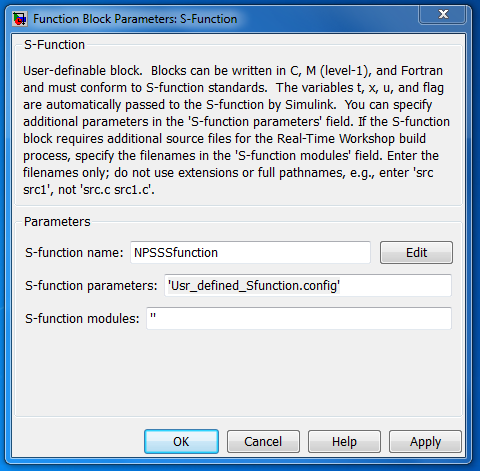
\includegraphics[width=0.5\textwidth]{images/SFuncDialog}
\caption{S Function Parameter Dialog Box}
\label{f:DialogBox}
\end{figure}

Where the configuration bash file includes all necessary paths, global envinronment variables, and specifies
which engine variables to expose to Simulink. This file defines the engine application program interface (API).

 \begin{adjustwidth}{-1cm}{-1cm}
 \inputminted[]{bash}{code/engineConfig.bat}
 \end{adjustwidth} 

This particular example includes multiple folders on the path for the NPSS distribution itself,
as well as paths within the engine folder.
The final command line string runs a batch run file and two optional preprocessor flags called \texttt{DFlag1}
and \texttt{DFlag2}. If not explicity added to the config file, the \texttt{engine.run} file must also set
the \texttt{NPSS\_TOP}, \texttt{NPSS\_DEV\_TOP}, \texttt{NPSS\_CONFIG}, and \texttt{NPSS\_TOP} environmental variables.

In this example, the config file will create an S-function block with 1 input port,
and 2 output ports each containing 5 muxed signals.
Signals fed into this input port will continuously update the value of the NPSS defined \texttt{Burner.Wfuel}
variable during the transient exectution. Similarly, all the specified outputs will be fed as output
signals of the Simulink block.
Multiple variables defined within a single ouptut port are muxed into a single signal bus.


In-depth examples of the S-functionc an be found in the source code for the
Tool for Turbine Engine Closed-loop Transient Analysis program (TTECTrA). \cite{TTECTrA}
The S-function was used extensively for this project under
NASA's Advanced Air Transportation Technologies (AATT) Project.

\section{Source-to-Source Translation}

The most abstract method of generating a transient model from NPSS is best described as ``Source-to-Source Translation"
(SST), which is the process of converting one high level model to another. This pattern is appropriate when developing
a transient engine model that may be completely separate, but originally derived, from NPSS.


(Possibly include TMATS?)

	Under the NASA Fundamental Aeronautics Program, the High Speed Project is developing a dynamic engine model
to better understand the coupling between propulsion and  aero-servo-elastic modes of long slender
supersonic vehicles. (Connolly, Kopasakis, \& Lemon, 2010) The supersonic component engine model (SCEM) is 
designed to extend a steady-state NPSS model and better capture high bandwidth dynamics associated with large
component volumes. The simulations aims to improve stability margin estimations and design engine control schedules
for compressor and exit nozzles of a variable cycle engine. Development of such a simulation can be challenging,
largely due to the number of engine components involved. Many of the challenges have been associated with data
management issues or difficulties in adaptability as the simulation has been scaled up in fidelity and engine complexity. 
Much like the intermediate fidelity model described in figure \ref{f:product_vs_time}, the SCEM model performs its
own unique calculations, but requires the steady-state engine characteristics of an existing NPSS model to initialize
the simulation. Source-to-source translation is one way to automate the conversion of an NPSS engine to help
reduce development time and alleviate model complexity.

\subsubsection{Problem Decomposition}

Although the SCEM solver is fundamentally different than the solver used by NPSS, both models are comprised of 
the same thermodynamic elements, linked together in the same order. Historically, the SCEM model has been
built up manually, element-by-element within Simulink based on the NPSS model architecture. Flow station properties
and performance maps generated by NPSS are saved into the Matlab workspace in large multi-dimensional matrices
and used to initialize the transient model. In order to automate the generation of an analogous SCEM model, the
program needs to adopt the same object-oriented nature of NPSS. By aligning the framework
paradigms between NPSS and SCEM, it is possible to create a parallel Matlab “objects” for each
standard element contained within NPSS. These Matlab objects contain all of the data book-keeping,
calculations and Simulink structures necessary to build many of the common elements within NPSS.
This automates the conversion of any NPSS model into an analogous Matlab model, greatly reducing
the opportunity for human error and simplifying the process of extending the model. The implementation
details for these Matlab objects are described in detail in subsequent sections of this report.	


\subsubsection{Program Goals and Future Development}

The automated Matlab/Simulink code generator was originally designed to aid in the construction of
the VCE engine for the APSE project; nonetheless it can theoretically be applied to any NPSS
model. As long as NPSS provides a consistent method for passing information, a Matlab object can
be created for every NPSS element and beyond. In order for the code generation tool to be useful
it will need to be as flexible as NPSS. The object-oriented nature will hopefully make this easy
by providing well-defined interfaces between the various component objects for developers, while
hiding the unnecessary implementation details from the user. The modularity of each element will
allow the program to be updated incrementally, and conversely, large program-wide changes can be
implemented simultaneously for all elements of the same type. 
	A second revision of the program will hopefully allow it to dynamically communicate with NPSS
providing balanced engine calculations on demand. A closer integration would eliminate the need
for large interpolation tables, allow for better suited data transfer and possibly increase the
speed and accuracy of the program.

\subsection{NPSS Implementation}

NPSS engine models vary widely in file organization and implementation details depending on the
model builder. The core commonality between models is the standard set of engine components and
the fluid and socket connections made between them. The custom functions created for this tool are
designed to be non-intrusive, and compatible with the wide variety of programming styles used to
build an NPSS model. The functions can easily be appended to existing models and only require a
small amount of user input to provide MATLAB with information that can’t be gleaned automatically.
All NPSS output is user-defined, so these custom functions were created to output engine data in a
format easily manipulated by Matlab and indexed in a manner that is still human-readable. The
three custom functions and their output are described below.

\subsubsection{NPSS to Matlab Run File}

After constructing the notional engine architecture in NPSS, run files are used to carry out
calculations and direct workflow in engine resizing, analysis and optimization. A MATLAB specific
run file was created to be appended to existing run files, allowing the engine to be run through
all the operating conditions of interest and output files to be used by MATLAB. The script sets
the appropriate independents/dependents to solve the simulation and then runs a single design
point to size the engine. Next, a series of off-design conditions are run to create a large matrix
of possible operating conditions across the flight envelope. A WATE++ model is then run to
generate the corresponding physical engine design. All of the pertinent information is then output
to MATLAB files. The MATLAB run file also includes an optional file that can be generated by
MATLAB before NPSS runs. This allows a user in the MATLAB environment to specify flight envelope
run cases of interest, then run NPSS all from within the MATLAB workspace. More information on the
workflow to pass from MATLAB to NPSS back to MATLAB can be found in the “Run NPSS” section of the
Matlab implementation section.

\subsection{Matlab Implementation}

\subsubsection{Component Library}

Similar to NPSS, a library of generic engine elements was composed to handle many combinations and
engine architectures. These custom Matlab classes use object-oriented features that first became
available in the R2008a revision of Matlab (The MathWorks Inc, R2013a), a language that primarily
supports a more procedural programming paradigm. An object is a specific instance of a class,
which follows the basic blueprint of the class, but with its own internal properties. Each
component class is complimented by a generic Simulink subsystem model. When an object is
instantiated and loaded, the component subsystem is added to the overall Simulink model. Each
class “book-keeps” data pertinent to that component type, and controls the behavior of the loaded
Simulink model. These classes help to keep the otherwise unwieldy amount of incoming data
organized, and allow the engine to be constructed automatically based on an equivalent NPSS
engine. Using a relatively small number of instructions (automatically generated by the NPSS
output described above) an entire Simulink engine can be constructed from various component
instances, be fully connected to each other, with every subsystem appropriately populated.

	The inherent modularity of the component library allows new classes to be added or modified
without affecting the rest of the library, while simultaneously allowing modifications to be made
across every instance of a particular class without duplicated effort. A system-wide bug affecting
every duct element in an engine could be addressed in a single piece of code, while still offering
the ability to tailor individual instances of ducts with various configurations and attributes.

\section{Final Remarks}
This is conclusions section it's quite handy.


\end{document}

%%% Local Variables: 
%%% mode: latex
%%% TeX-master: t
%%% End: 
